% generated by paper/make_figures.py from results/rev3 - do not edit
\appendix
\section{Supplementary Measurement Figures}
\label{app:figs}
Figs.~\ref{fig:app-tcp}--\ref{fig:app-newconn} plot the measurements behind Tables~\ref{tab:perf} and \ref{tab:paths} with their 95\% confidence intervals (Student $t$). Value axes are zoomed so that the intervals are visible; each caption gives the axis origin, and differences between bars should be judged against the intervals, not against the axis origin. In-kernel panels show the first of the three microbenchmark runs with its within-run intervals; Table~\ref{tab:paths} and Fig.~\ref{fig:scale} give the mean and range over all three. Table~\ref{tab:figindex} lists every figure with its quantity, the configurations it covers and its data file in the results directory (\texttt{results/rev3}).

\begin{table}[!h]
\caption{Index of the supplementary figures}
\label{tab:figindex}
\centering\scriptsize
\setlength{\tabcolsep}{3pt}
\begin{tabular}{@{}rlll@{}}
\toprule
Fig. & Name & Unit & Configurations \\
\midrule
\ref{fig:app-tcp} & Routed TCP throughput & Gbit/s & all \\
\ref{fig:app-pps} & Routed packet rate & kpps & all \\
\ref{fig:app-viptcp} & VIP TCP throughput & Gbit/s & LB-capable \\
\ref{fig:app-vippps} & VIP packet rate & kpps & LB-capable \\
\ref{fig:app-rulestcp} & Populated rules, TCP & Gbit/s & five stateful \\
\ref{fig:app-rulespps} & Populated rules, packet rate & kpps & five stateful \\
\ref{fig:app-vskernel} & Paired difference to Kernel & \% & all \\
\ref{fig:app-vsovs} & Paired difference to OVS-ct & \% & LB-capable \\
\ref{fig:app-rtt} & Average RTT & $\mu$s & all \\
\ref{fig:app-lbrps} & VIP connection rate & conn./s & LB-capable \\
\ref{fig:app-paths} & Per-path cost by hook & ns & XDP, TC \\
\ref{fig:app-cold} & Cache-cold cost & ns & XDP, TC \\
\ref{fig:app-chain} & Tail-call ablation & ns & XDP \\
\ref{fig:app-newconn} & New-connection cost & ns & XDP, TC \\
\bottomrule
\end{tabular}
\\[2pt]
\parbox{\columnwidth}{\footnotesize Macro-benchmark data: \texttt{rev3/<cfg>.json} (10 interleaved rounds). In-kernel data: \texttt{rev4/microbench\_1.json}.}
\end{table}

\begin{figure*}[!p]\centering
\begin{minipage}[t]{0.48\textwidth}\centering
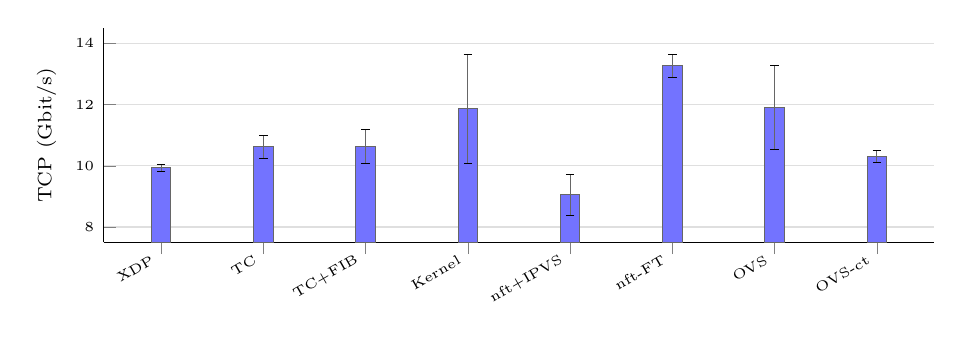
\begin{tikzpicture}
\begin{axis}[ybar, width=\linewidth, height=4.3cm, bar width=7pt,
  scaled y ticks=false, yticklabel style={/pgf/number format/fixed},
  symbolic x coords={XDP,TC,TC+FIB,Kernel,nft+IPVS,nft-FT,OVS,OVS-ct}, xtick=data, ymin=7.5, ymax=14.5,
  ylabel={TCP (Gbit/s)}, enlarge x limits=0.08, axis lines*=left,
  ymajorgrids, grid style={gray!25}, x tick label style={rotate=30, anchor=east, font=\tiny},
  y tick label style={font=\tiny}, label style={font=\scriptsize},
  error bars/y dir=both, error bars/y explicit]
\addplot[fill=blue!55, draw=black!60, error bars/.cd, y dir=both, y explicit, error mark options={rotate=90, mark size=1.5pt}] coordinates {(XDP,9.939) +- (0,0.117) (TC,10.62) +- (0,0.386) (TC+FIB,10.63) +- (0,0.555) (Kernel,11.87) +- (0,1.78) (nft+IPVS,9.057) +- (0,0.669) (nft-FT,13.27) +- (0,0.383) (OVS,11.9) +- (0,1.38) (OVS-ct,10.3) +- (0,0.204)};
\end{axis}
\end{tikzpicture}
\captionof{figure}{\textbf{Routed TCP throughput.} Routed-path TCP throughput, mean $\pm$ 95\% CI over 10 interleaved rounds. Axis starts at 7.5.}\label{fig:app-tcp}
\end{minipage}
\hfill
\begin{minipage}[t]{0.48\textwidth}\centering
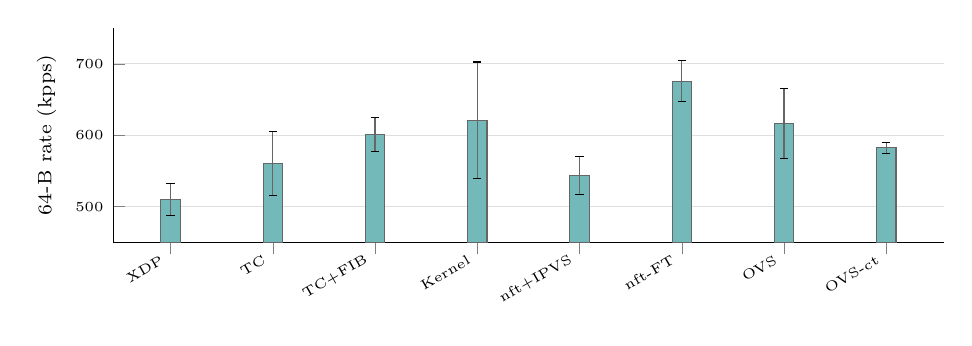
\begin{tikzpicture}
\begin{axis}[ybar, width=\linewidth, height=4.3cm, bar width=7pt,
  scaled y ticks=false, yticklabel style={/pgf/number format/fixed},
  symbolic x coords={XDP,TC,TC+FIB,Kernel,nft+IPVS,nft-FT,OVS,OVS-ct}, xtick=data, ymin=450, ymax=750,
  ylabel={64-B rate (kpps)}, enlarge x limits=0.08, axis lines*=left,
  ymajorgrids, grid style={gray!25}, x tick label style={rotate=30, anchor=east, font=\tiny},
  y tick label style={font=\tiny}, label style={font=\scriptsize},
  error bars/y dir=both, error bars/y explicit]
\addplot[fill=teal!55, draw=black!60, error bars/.cd, y dir=both, y explicit, error mark options={rotate=90, mark size=1.5pt}] coordinates {(XDP,510.2) +- (0,22.7) (TC,560.4) +- (0,45.1) (TC+FIB,601.5) +- (0,23.8) (Kernel,620.9) +- (0,81.7) (nft+IPVS,543.7) +- (0,26.3) (nft-FT,675.5) +- (0,28.8) (OVS,616.4) +- (0,48.8) (OVS-ct,582.4) +- (0,7.66)};
\end{axis}
\end{tikzpicture}
\captionof{figure}{\textbf{Routed packet rate.} Routed-path 64-byte packet rate, mean $\pm$ 95\% CI over 10 interleaved rounds. Axis starts at 450.}\label{fig:app-pps}
\end{minipage}
\par\vspace{2mm}
\begin{minipage}[t]{0.48\textwidth}\centering
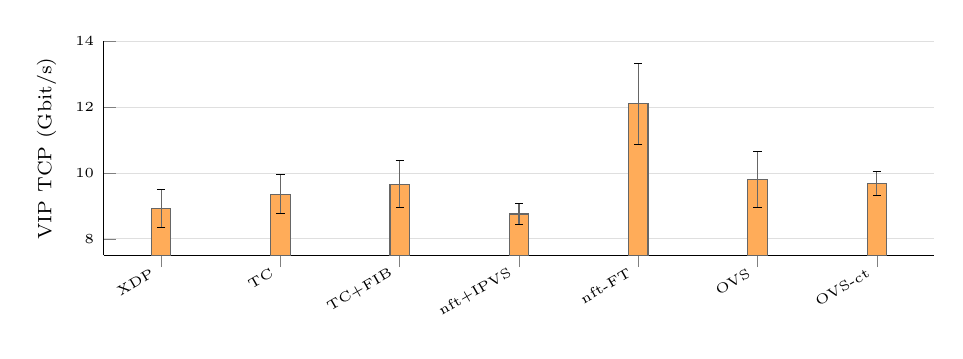
\begin{tikzpicture}
\begin{axis}[ybar, width=\linewidth, height=4.3cm, bar width=7pt,
  scaled y ticks=false, yticklabel style={/pgf/number format/fixed},
  symbolic x coords={XDP,TC,TC+FIB,nft+IPVS,nft-FT,OVS,OVS-ct}, xtick=data, ymin=7.5, ymax=14,
  ylabel={VIP TCP (Gbit/s)}, enlarge x limits=0.08, axis lines*=left,
  ymajorgrids, grid style={gray!25}, x tick label style={rotate=30, anchor=east, font=\tiny},
  y tick label style={font=\tiny}, label style={font=\scriptsize},
  error bars/y dir=both, error bars/y explicit]
\addplot[fill=orange!65, draw=black!60, error bars/.cd, y dir=both, y explicit, error mark options={rotate=90, mark size=1.5pt}] coordinates {(XDP,8.921) +- (0,0.568) (TC,9.36) +- (0,0.599) (TC+FIB,9.664) +- (0,0.709) (nft+IPVS,8.758) +- (0,0.308) (nft-FT,12.1) +- (0,1.23) (OVS,9.814) +- (0,0.85) (OVS-ct,9.671) +- (0,0.364)};
\end{axis}
\end{tikzpicture}
\captionof{figure}{\textbf{VIP TCP throughput.} TCP throughput through the load balancer (VIP path), mean $\pm$ 95\% CI over 10 interleaved rounds. Axis starts at 7.5.}\label{fig:app-viptcp}
\end{minipage}
\hfill
\begin{minipage}[t]{0.48\textwidth}\centering
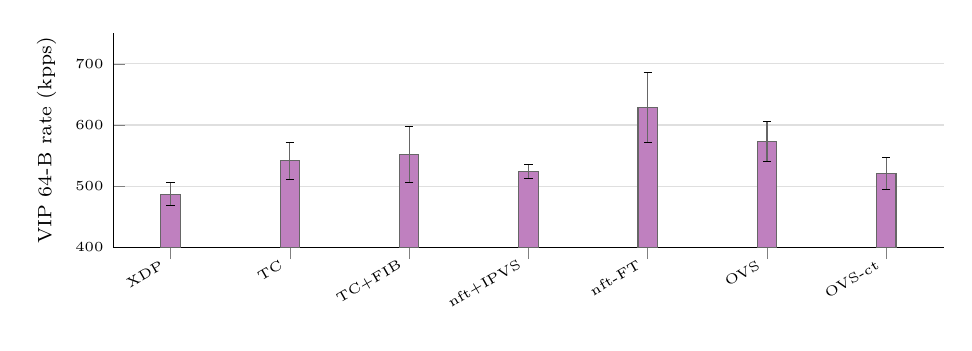
\begin{tikzpicture}
\begin{axis}[ybar, width=\linewidth, height=4.3cm, bar width=7pt,
  scaled y ticks=false, yticklabel style={/pgf/number format/fixed},
  symbolic x coords={XDP,TC,TC+FIB,nft+IPVS,nft-FT,OVS,OVS-ct}, xtick=data, ymin=400, ymax=750,
  ylabel={VIP 64-B rate (kpps)}, enlarge x limits=0.08, axis lines*=left,
  ymajorgrids, grid style={gray!25}, x tick label style={rotate=30, anchor=east, font=\tiny},
  y tick label style={font=\tiny}, label style={font=\scriptsize},
  error bars/y dir=both, error bars/y explicit]
\addplot[fill=violet!50, draw=black!60, error bars/.cd, y dir=both, y explicit, error mark options={rotate=90, mark size=1.5pt}] coordinates {(XDP,487.1) +- (0,19.1) (TC,541.4) +- (0,30.1) (TC+FIB,551.8) +- (0,46) (nft+IPVS,523.8) +- (0,11.7) (nft-FT,628.2) +- (0,57.2) (OVS,573.4) +- (0,32.4) (OVS-ct,520.9) +- (0,26.1)};
\end{axis}
\end{tikzpicture}
\captionof{figure}{\textbf{VIP packet rate.} 64-byte packet rate through the load balancer, mean $\pm$ 95\% CI over 10 interleaved rounds. Axis starts at 400.}\label{fig:app-vippps}
\end{minipage}
\par\vspace{2mm}
\begin{minipage}[t]{0.48\textwidth}\centering
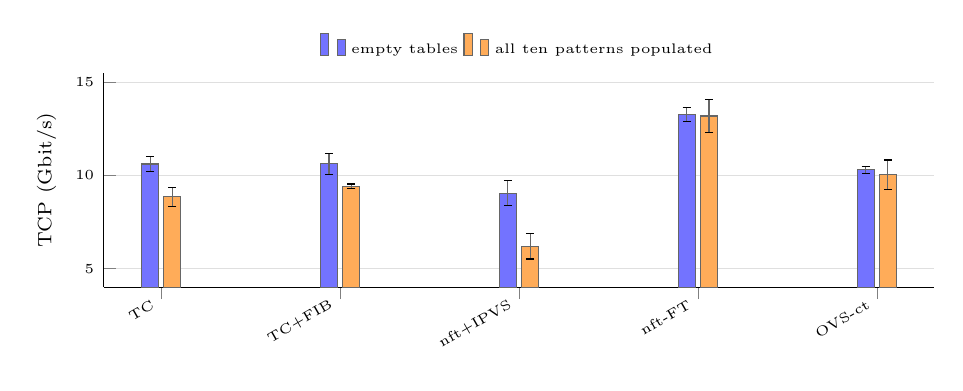
\begin{tikzpicture}
\begin{axis}[ybar, width=\linewidth, height=4.3cm, bar width=7pt,
  scaled y ticks=false, yticklabel style={/pgf/number format/fixed},
  symbolic x coords={TC,TC+FIB,nft+IPVS,nft-FT,OVS-ct}, xtick=data, ymin=4, ymax=15.5,
  ylabel={TCP (Gbit/s)}, enlarge x limits=0.08, axis lines*=left,
  ymajorgrids, grid style={gray!25}, x tick label style={rotate=30, anchor=east, font=\tiny},
  y tick label style={font=\tiny}, label style={font=\scriptsize},
  error bars/y dir=both, error bars/y explicit, bar width=6pt, legend style={font=\tiny, at={(0.5,1.02)}, anchor=south, legend columns=2, draw=none}]
\addplot[fill=blue!55, draw=black!60, error bars/.cd, y dir=both, y explicit, error mark options={rotate=90, mark size=1.5pt}] coordinates {(TC,10.62) +- (0,0.386) (TC+FIB,10.63) +- (0,0.555) (nft+IPVS,9.057) +- (0,0.669) (nft-FT,13.27) +- (0,0.383) (OVS-ct,10.3) +- (0,0.204)};
\addplot[fill=orange!65, draw=black!60, error bars/.cd, y dir=both, y explicit, error mark options={rotate=90, mark size=1.5pt}] coordinates {(TC,8.852) +- (0,0.51) (TC+FIB,9.419) +- (0,0.127) (nft+IPVS,6.202) +- (0,0.688) (nft-FT,13.2) +- (0,0.869) (OVS-ct,10.04) +- (0,0.792)};
\legend{empty tables, all ten patterns populated}
\end{axis}
\end{tikzpicture}
\captionof{figure}{\textbf{Populated rules, TCP.} Routed TCP throughput with empty rule tables and with 1000 rules populating all ten patterns, mean $\pm$ 95\% CI over 10 interleaved rounds. Axis starts at 4.}\label{fig:app-rulestcp}
\end{minipage}
\hfill
\begin{minipage}[t]{0.48\textwidth}\centering
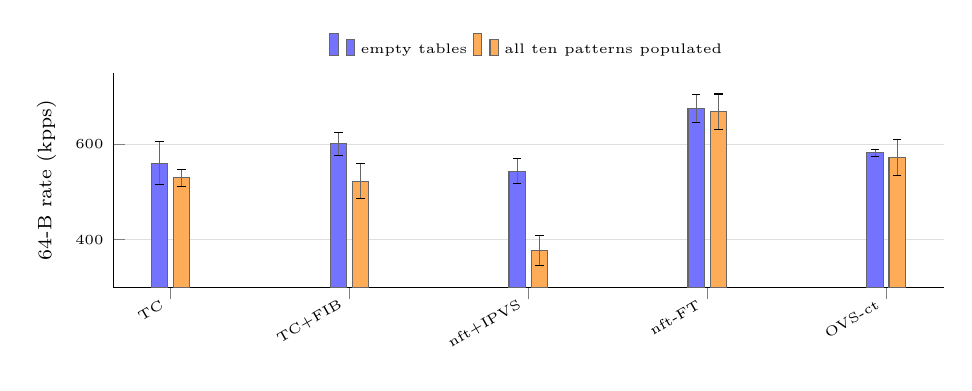
\begin{tikzpicture}
\begin{axis}[ybar, width=\linewidth, height=4.3cm, bar width=7pt,
  scaled y ticks=false, yticklabel style={/pgf/number format/fixed},
  symbolic x coords={TC,TC+FIB,nft+IPVS,nft-FT,OVS-ct}, xtick=data, ymin=300, ymax=750,
  ylabel={64-B rate (kpps)}, enlarge x limits=0.08, axis lines*=left,
  ymajorgrids, grid style={gray!25}, x tick label style={rotate=30, anchor=east, font=\tiny},
  y tick label style={font=\tiny}, label style={font=\scriptsize},
  error bars/y dir=both, error bars/y explicit, bar width=6pt, legend style={font=\tiny, at={(0.5,1.02)}, anchor=south, legend columns=2, draw=none}]
\addplot[fill=blue!55, draw=black!60, error bars/.cd, y dir=both, y explicit, error mark options={rotate=90, mark size=1.5pt}] coordinates {(TC,560.4) +- (0,45.1) (TC+FIB,601.5) +- (0,23.8) (nft+IPVS,543.7) +- (0,26.3) (nft-FT,675.5) +- (0,28.8) (OVS-ct,582.4) +- (0,7.66)};
\addplot[fill=orange!65, draw=black!60, error bars/.cd, y dir=both, y explicit, error mark options={rotate=90, mark size=1.5pt}] coordinates {(TC,529.8) +- (0,17.7) (TC+FIB,523.1) +- (0,37) (nft+IPVS,377.1) +- (0,31.7) (nft-FT,669.2) +- (0,37) (OVS-ct,572.5) +- (0,38.1)};
\legend{empty tables, all ten patterns populated}
\end{axis}
\end{tikzpicture}
\captionof{figure}{\textbf{Populated rules, packet rate.} Routed 64-byte packet rate with empty and populated rule tables, mean $\pm$ 95\% CI over 10 interleaved rounds. Axis starts at 300.}\label{fig:app-rulespps}
\end{minipage}
\par\vspace{2mm}
\begin{minipage}[t]{0.48\textwidth}\centering
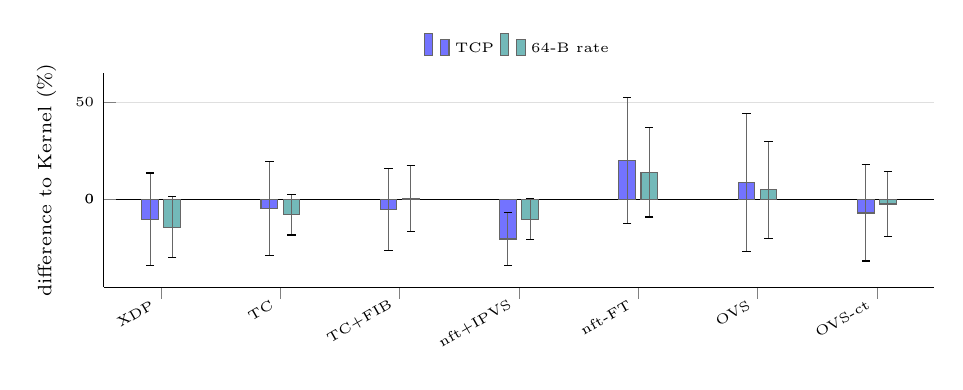
\begin{tikzpicture}
\begin{axis}[ybar, width=\linewidth, height=4.3cm, bar width=7pt,
  scaled y ticks=false, yticklabel style={/pgf/number format/fixed},
  symbolic x coords={XDP,TC,TC+FIB,nft+IPVS,nft-FT,OVS,OVS-ct}, xtick=data, ymin=-45, ymax=65,
  ylabel={difference to Kernel (\%)}, enlarge x limits=0.08, axis lines*=left,
  ymajorgrids, grid style={gray!25}, x tick label style={rotate=30, anchor=east, font=\tiny},
  y tick label style={font=\tiny}, label style={font=\scriptsize},
  error bars/y dir=both, error bars/y explicit, bar width=6pt, legend style={font=\tiny, at={(0.5,1.02)}, anchor=south, legend columns=2, draw=none}, extra y ticks={0}, extra y tick style={grid style={black, thin}}]
\addplot[fill=blue!55, draw=black!60, error bars/.cd, y dir=both, y explicit, error mark options={rotate=90, mark size=1.5pt}] coordinates {(XDP,-10.15) +- (0,23.8) (TC,-4.453) +- (0,24.1) (TC+FIB,-4.985) +- (0,21) (nft+IPVS,-20.31) +- (0,13.5) (nft-FT,20.01) +- (0,32.2) (OVS,8.885) +- (0,35.5) (OVS-ct,-6.903) +- (0,24.7)};
\addplot[fill=teal!55, draw=black!60, error bars/.cd, y dir=both, y explicit, error mark options={rotate=90, mark size=1.5pt}] coordinates {(XDP,-14.25) +- (0,15.7) (TC,-7.713) +- (0,10.5) (TC+FIB,0.6934) +- (0,16.9) (nft+IPVS,-10.04) +- (0,10.5) (nft-FT,14.02) +- (0,23) (OVS,4.938) +- (0,25.1) (OVS-ct,-2.314) +- (0,16.9)};
\legend{TCP, 64-B rate}
\end{axis}
\end{tikzpicture}
\captionof{figure}{\textbf{Paired difference to Kernel.} Performance relative to plain kernel routing (negative: slower): per-round paired relative difference over all 10 rounds, including kernel routing's outlier round~8, mean $\pm$ 95\% CI (paired $t$). Axis from -45 to 65\,\%.}\label{fig:app-vskernel}
\end{minipage}
\hfill
\begin{minipage}[t]{0.48\textwidth}\centering
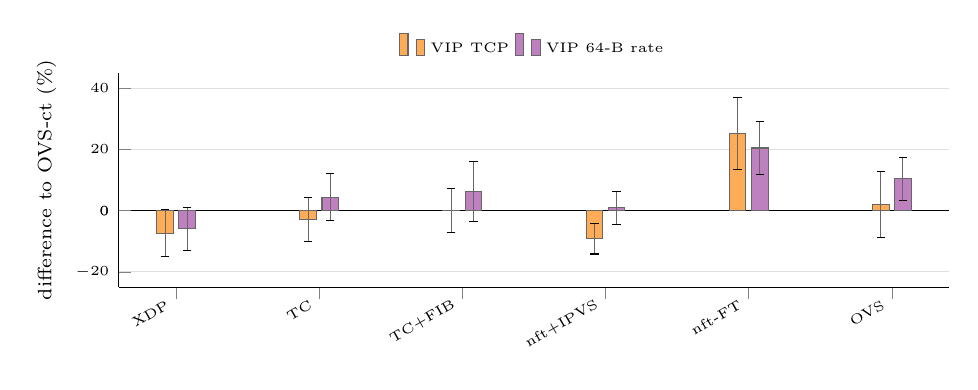
\begin{tikzpicture}
\begin{axis}[ybar, width=\linewidth, height=4.3cm, bar width=7pt,
  scaled y ticks=false, yticklabel style={/pgf/number format/fixed},
  symbolic x coords={XDP,TC,TC+FIB,nft+IPVS,nft-FT,OVS}, xtick=data, ymin=-25, ymax=45,
  ylabel={difference to OVS-ct (\%)}, enlarge x limits=0.08, axis lines*=left,
  ymajorgrids, grid style={gray!25}, x tick label style={rotate=30, anchor=east, font=\tiny},
  y tick label style={font=\tiny}, label style={font=\scriptsize},
  error bars/y dir=both, error bars/y explicit, bar width=6pt, legend style={font=\tiny, at={(0.5,1.02)}, anchor=south, legend columns=2, draw=none}, extra y ticks={0}, extra y tick style={grid style={black, thin}}]
\addplot[fill=orange!65, draw=black!60, error bars/.cd, y dir=both, y explicit, error mark options={rotate=90, mark size=1.5pt}] coordinates {(XDP,-7.4) +- (0,7.72) (TC,-2.982) +- (0,7.14) (TC+FIB,0.03369) +- (0,7.09) (nft+IPVS,-9.206) +- (0,4.97) (nft-FT,25.12) +- (0,11.8) (OVS,1.923) +- (0,10.8)};
\addplot[fill=violet!50, draw=black!60, error bars/.cd, y dir=both, y explicit, error mark options={rotate=90, mark size=1.5pt}] coordinates {(XDP,-5.955) +- (0,7.02) (TC,4.358) +- (0,7.69) (TC+FIB,6.33) +- (0,9.79) (nft+IPVS,0.9904) +- (0,5.38) (nft-FT,20.48) +- (0,8.72) (OVS,10.4) +- (0,7.12)};
\legend{VIP TCP, VIP 64-B rate}
\end{axis}
\end{tikzpicture}
\captionof{figure}{\textbf{Paired difference to OVS-ct.} VIP-path performance relative to OVS-ct: per-round paired relative difference, mean $\pm$ 95\% CI (paired $t$). Axis from -25 to 45\,\%.}\label{fig:app-vsovs}
\end{minipage}
\end{figure*}
\begin{figure*}[!p]\centering
\begin{minipage}[t]{0.48\textwidth}\centering
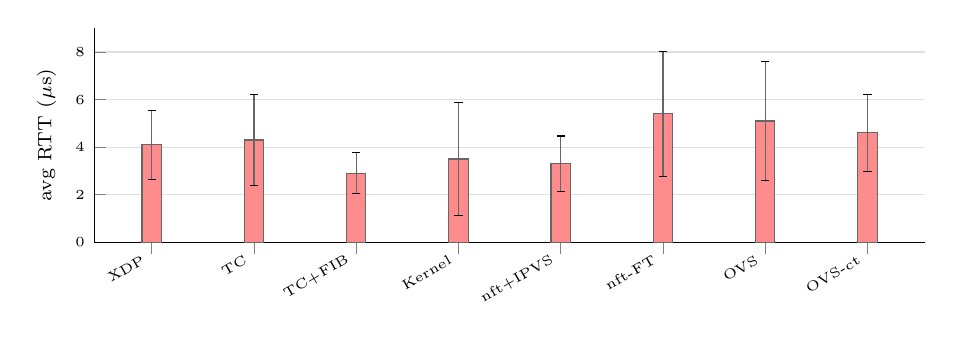
\begin{tikzpicture}
\begin{axis}[ybar, width=\linewidth, height=4.3cm, bar width=7pt,
  scaled y ticks=false, yticklabel style={/pgf/number format/fixed},
  symbolic x coords={XDP,TC,TC+FIB,Kernel,nft+IPVS,nft-FT,OVS,OVS-ct}, xtick=data, ymin=0, ymax=9,
  ylabel={avg RTT ($\mu$s)}, enlarge x limits=0.08, axis lines*=left,
  ymajorgrids, grid style={gray!25}, x tick label style={rotate=30, anchor=east, font=\tiny},
  y tick label style={font=\tiny}, label style={font=\scriptsize},
  error bars/y dir=both, error bars/y explicit]
\addplot[fill=red!45, draw=black!60, error bars/.cd, y dir=both, y explicit, error mark options={rotate=90, mark size=1.5pt}] coordinates {(XDP,4.1) +- (0,1.45) (TC,4.3) +- (0,1.91) (TC+FIB,2.9) +- (0,0.856) (Kernel,3.5) +- (0,2.37) (nft+IPVS,3.3) +- (0,1.17) (nft-FT,5.4) +- (0,2.64) (OVS,5.1) +- (0,2.51) (OVS-ct,4.6) +- (0,1.62)};
\end{axis}
\end{tikzpicture}
\captionof{figure}{\textbf{Average RTT.} Average round-trip time on the routed path, mean $\pm$ 95\% CI over 10 interleaved rounds. Axis starts at 0.}\label{fig:app-rtt}
\end{minipage}
\hfill
\begin{minipage}[t]{0.48\textwidth}\centering
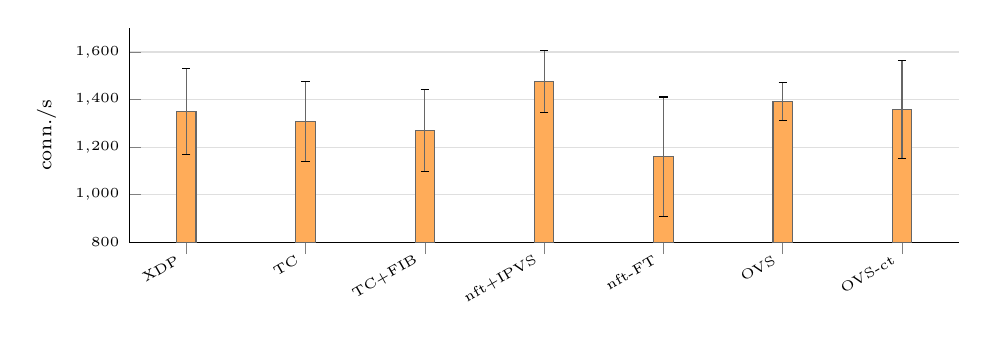
\begin{tikzpicture}
\begin{axis}[ybar, width=\linewidth, height=4.3cm, bar width=7pt,
  scaled y ticks=false, yticklabel style={/pgf/number format/fixed},
  symbolic x coords={XDP,TC,TC+FIB,nft+IPVS,nft-FT,OVS,OVS-ct}, xtick=data, ymin=800, ymax=1700,
  ylabel={conn./s}, enlarge x limits=0.08, axis lines*=left,
  ymajorgrids, grid style={gray!25}, x tick label style={rotate=30, anchor=east, font=\tiny},
  y tick label style={font=\tiny}, label style={font=\scriptsize},
  error bars/y dir=both, error bars/y explicit]
\addplot[fill=orange!65, draw=black!60, error bars/.cd, y dir=both, y explicit, error mark options={rotate=90, mark size=1.5pt}] coordinates {(XDP,1349) +- (0,180) (TC,1308) +- (0,169) (TC+FIB,1269) +- (0,172) (nft+IPVS,1476) +- (0,131) (nft-FT,1159) +- (0,252) (OVS,1393) +- (0,79.7) (OVS-ct,1359) +- (0,206)};
\end{axis}
\end{tikzpicture}
\captionof{figure}{\textbf{VIP connection rate.} New-connection rate through the VIP (HTTP), mean $\pm$ 95\% CI over 10 interleaved rounds. Axis starts at 800.}\label{fig:app-lbrps}
\end{minipage}
\par\vspace{2mm}
\begin{minipage}[t]{0.48\textwidth}\centering
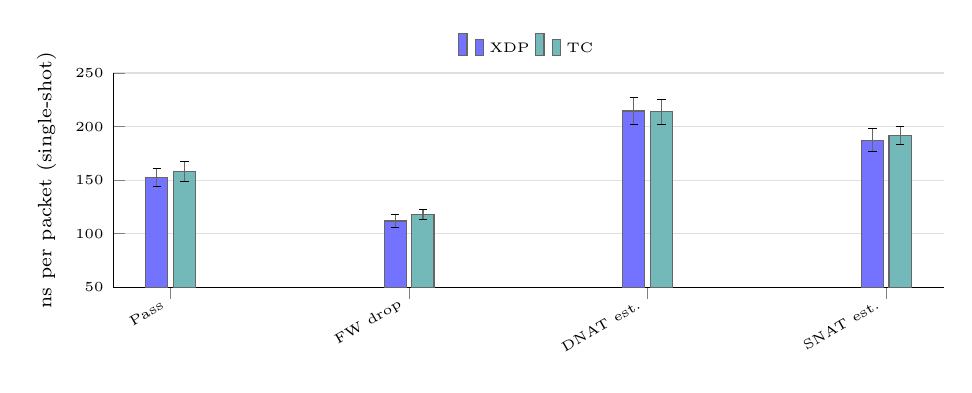
\begin{tikzpicture}
\begin{axis}[ybar, width=\linewidth, height=4.3cm, bar width=7pt,
  scaled y ticks=false, yticklabel style={/pgf/number format/fixed},
  symbolic x coords={Pass,FW drop,DNAT est.,SNAT est.}, xtick=data, ymin=50, ymax=250,
  ylabel={ns per packet (single-shot)}, enlarge x limits=0.08, axis lines*=left,
  ymajorgrids, grid style={gray!25}, x tick label style={rotate=30, anchor=east, font=\tiny},
  y tick label style={font=\tiny}, label style={font=\scriptsize},
  error bars/y dir=both, error bars/y explicit, bar width=8pt, legend style={font=\tiny, at={(0.5,1.02)}, anchor=south, legend columns=2, draw=none}]
\addplot[fill=blue!55, draw=black!60, error bars/.cd, y dir=both, y explicit, error mark options={rotate=90, mark size=1.5pt}] coordinates {(Pass,152.2) +- (0,8.34) (FW drop,111.8) +- (0,6.16) (DNAT est.,214.5) +- (0,12.5) (SNAT est.,187.1) +- (0,10.8)};
\addplot[fill=teal!55, draw=black!60, error bars/.cd, y dir=both, y explicit, error mark options={rotate=90, mark size=1.5pt}] coordinates {(Pass,158.2) +- (0,9.54) (FW drop,117.9) +- (0,4.96) (DNAT est.,213.8) +- (0,11.5) (SNAT est.,191.4) +- (0,8.3)};
\legend{XDP, TC}
\end{axis}
\end{tikzpicture}
\captionof{figure}{\textbf{Per-path cost by hook.} In-kernel single-shot cost per processing path at the XDP and TC hooks with one installed rule; mean $\pm$ 95\% CI of 10 batch means. Axis starts at 50.}\label{fig:app-paths}
\end{minipage}
\hfill
\begin{minipage}[t]{0.48\textwidth}\centering
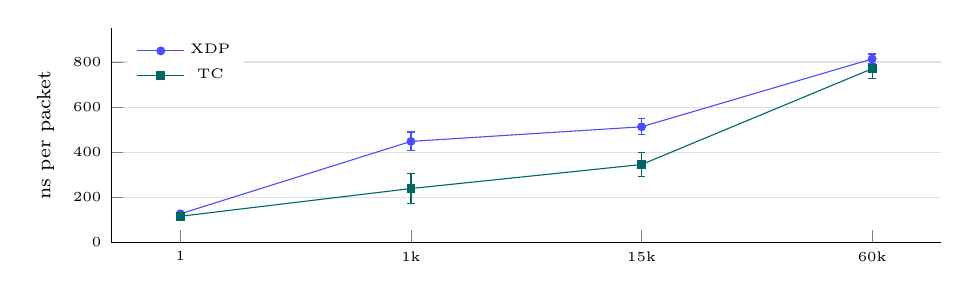
\begin{tikzpicture}
\begin{axis}[width=\linewidth, height=4.3cm, scaled y ticks=false, symbolic x coords={1,1k,15k,60k}, xtick=data, ymin=0, ymax=950, ylabel={ns per packet},
  axis lines*=left, ymajorgrids, grid style={gray!25}, tick label style={font=\tiny}, label style={font=\scriptsize},
  legend style={font=\tiny, at={(0.02,0.98)}, anchor=north west, draw=none}]
\addplot[blue!70, mark=*, mark size=1.4pt, error bars/.cd, y dir=both, y explicit] coordinates {(1,126.4) +- (0,1.85) (1k,447.8) +- (0,41.8) (15k,512.6) +- (0,34.8) (60k,813.9) +- (0,21.6)};
\addplot[teal!80!black, mark=square*, mark size=1.4pt, error bars/.cd, y dir=both, y explicit] coordinates {(1,115.5) +- (0,2.61) (1k,238.5) +- (0,65.1) (15k,345.2) +- (0,54.3) (60k,770.4) +- (0,43.2)};
\legend{XDP, TC}
\end{axis}
\end{tikzpicture}
\captionof{figure}{\textbf{Cache-cold cost.} In-kernel single-shot cost versus the number of tracked flows visited in random order (cache-cold, empty rule tables; 15k flows fit the 16\,384-entry telemetry table, 60k do not); mean $\pm$ 95\% CI of 10 batch means, first of three runs. Axis starts at 0.}\label{fig:app-cold}
\end{minipage}
\par\vspace{2mm}
\begin{minipage}[t]{0.48\textwidth}\centering
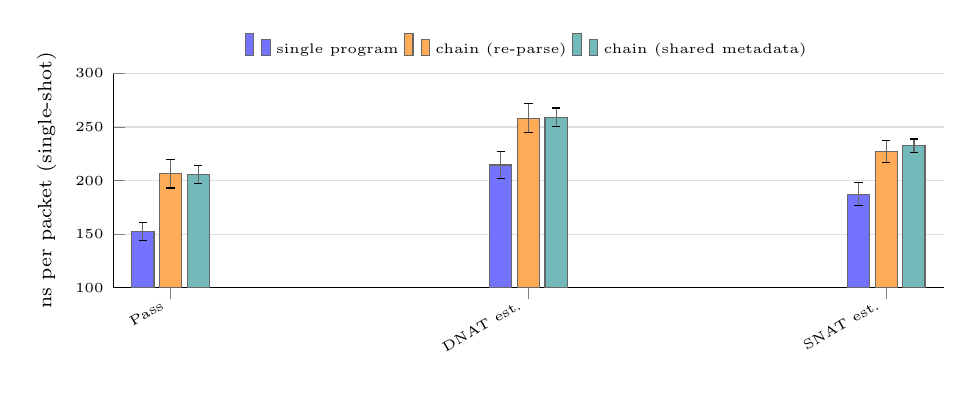
\begin{tikzpicture}
\begin{axis}[ybar, width=\linewidth, height=4.3cm, bar width=7pt,
  scaled y ticks=false, yticklabel style={/pgf/number format/fixed},
  symbolic x coords={Pass,DNAT est.,SNAT est.}, xtick=data, ymin=100, ymax=300,
  ylabel={ns per packet (single-shot)}, enlarge x limits=0.08, axis lines*=left,
  ymajorgrids, grid style={gray!25}, x tick label style={rotate=30, anchor=east, font=\tiny},
  y tick label style={font=\tiny}, label style={font=\scriptsize},
  error bars/y dir=both, error bars/y explicit, bar width=8pt, legend style={font=\tiny, at={(0.5,1.02)}, anchor=south, legend columns=3, draw=none}]
\addplot[fill=blue!55, draw=black!60, error bars/.cd, y dir=both, y explicit, error mark options={rotate=90, mark size=1.5pt}] coordinates {(Pass,152.2) +- (0,8.34) (DNAT est.,214.5) +- (0,12.5) (SNAT est.,187.1) +- (0,10.8)};
\addplot[fill=orange!65, draw=black!60, error bars/.cd, y dir=both, y explicit, error mark options={rotate=90, mark size=1.5pt}] coordinates {(Pass,206.5) +- (0,13.5) (DNAT est.,258.4) +- (0,13.8) (SNAT est.,227.2) +- (0,9.98)};
\addplot[fill=teal!55, draw=black!60, error bars/.cd, y dir=both, y explicit, error mark options={rotate=90, mark size=1.5pt}] coordinates {(Pass,205.3) +- (0,8.43) (DNAT est.,259.1) +- (0,8.68) (SNAT est.,232.5) +- (0,6.34)};
\legend{single program, chain (re-parse), chain (shared metadata)}
\end{axis}
\end{tikzpicture}
\captionof{figure}{\textbf{Tail-call ablation.} Tail-call ablation (XDP, single-shot): single program versus the same stages chained with tail calls, re-parsing in every stage or sharing the parse result through a per-CPU map; mean $\pm$ 95\% CI of 10 batch means, first of three runs. Axis starts at 100.}\label{fig:app-chain}
\end{minipage}
\hfill
\begin{minipage}[t]{0.48\textwidth}\centering
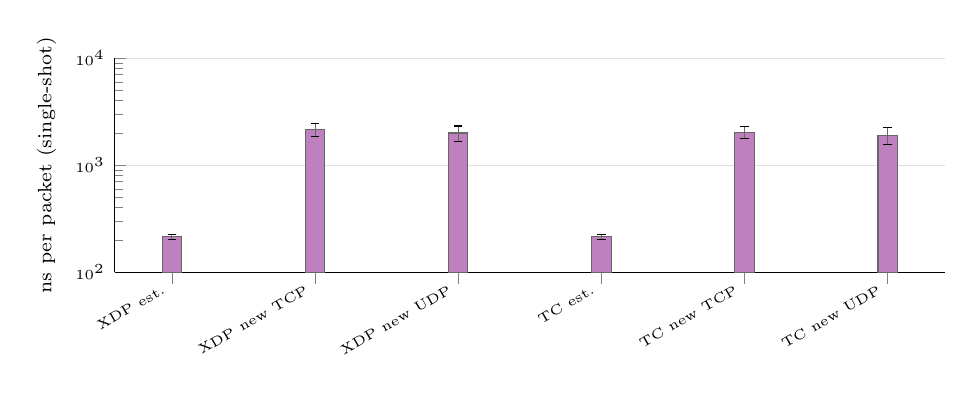
\begin{tikzpicture}
\begin{axis}[ybar, width=\linewidth, height=4.3cm, bar width=7pt,
  scaled y ticks=false, yticklabel style={/pgf/number format/fixed},
  symbolic x coords={XDP est.,XDP new TCP,XDP new UDP,TC est.,TC new TCP,TC new UDP}, xtick=data, ymin=100, ymax=10000,
  ylabel={ns per packet (single-shot)}, enlarge x limits=0.08, axis lines*=left,
  ymajorgrids, grid style={gray!25}, x tick label style={rotate=30, anchor=east, font=\tiny},
  y tick label style={font=\tiny}, label style={font=\scriptsize},
  error bars/y dir=both, error bars/y explicit, ymode=log, log origin=infty]
\addplot[fill=violet!50, draw=black!60, error bars/.cd, y dir=both, y explicit, error mark options={rotate=90, mark size=1.5pt}] coordinates {(XDP est.,214.5) +- (0,12.5) (XDP new TCP,2147) +- (0,290) (XDP new UDP,1996) +- (0,326) (TC est.,213.8) +- (0,11.5) (TC new TCP,2037) +- (0,271) (TC new UDP,1909) +- (0,346)};
\end{axis}
\end{tikzpicture}
\captionof{figure}{\textbf{New-connection cost.} In-kernel single-shot cost of DNAT for an established connection, a new TCP connection (the SYN deletes the $n=4$ reverse entries of the pool) and a new UDP flow (probes them); mean $\pm$ 95\% CI of 10 batch means, first of three runs. Logarithmic axis.}\label{fig:app-newconn}
\end{minipage}
\end{figure*}
\clearpage  % flush the figure pages before the references
